\documentclass{standalone}
\usepackage{tikz}
\usetikzlibrary{intersections}
\renewcommand{\familydefault}{\sfdefault}
\begin{document}
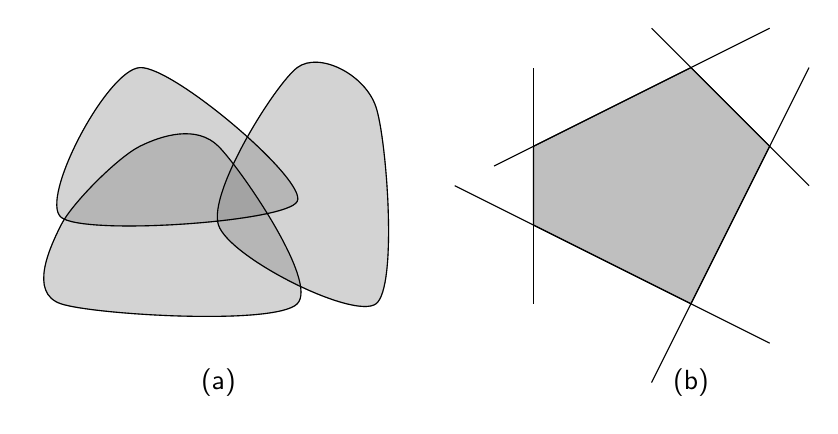
\begin{tikzpicture}
  \draw [fill = gray, opacity = .35] plot [smooth cycle] coordinates {(0,0) (1,1) (2,1) (3,-1) (0,-1)};
  \draw [fill = gray, opacity = .35] plot [smooth cycle] coordinates {(2,0) (3,2) (4, 1.5) (4, -1)};
  \draw [fill = gray, opacity = .35] plot [smooth cycle] coordinates {(1,2) (3,.3) (0, .1)};

  \draw plot [smooth cycle] coordinates {(0,0) (1,1) (2,1) (3,-1) (0,-1)};
  \draw  plot [smooth cycle] coordinates {(2,0) (3,2) (4, 1.5) (4, -1)};
  \draw  plot [smooth cycle] coordinates {(1,2) (3,.3) (0, .1)};

  \begin{scope}[xshift = 6cm]
  \draw [fill = gray!50] (0, 0)  --  (2, -1)  --  (3, 1)  --  (2, 2)  --  (0, 1)  --  cycle;
  
  \draw (-1, .5)  --  (3, -1.5);
  \draw (1.5, -2)  --  (3.5, 2);
  \draw (-.5, .75)  --  (3, 2.5);
  \draw (0, -1)  --  (0, 2);
  \draw (3.5, .5)  --  (1.5, 2.5);

  \node at (2, -2) {(b)};
  \node at (-4, -2) {(a)};
  \end{scope}
\end{tikzpicture}
\end{document} 